%-*-coding: utf-8-*-

\chapter{Сбор информации о приложении}
	В данной главе будут описаны подходы к решению задачи сбора информации о приложении. Также будут рассмотрены основные аспекты и сложности возникающие при ее решении. В конце будет показан анализ накладных расходов на профилируемое приложение. 

\section{Общий принцип работы}
	На рисунке \ref{fig:general_profiler} можно увидеть алгоритм работы, детали которого будут описаны в следующих секциях. Профайлер способен работать в двух режимах: 

\begin{enumerate}
	\item запуская программу
    \item подключаться к уже запущенному приложению
\end{enumerate}

	В первом режиме профайлер сам запускает программу посредством функции \verb|execvp(...)| и контролирует ее время жизни. Если профайлер будет остановлен по требованию пользователя, то он также завершит и выполнение профилируемой программы.
    
    Во втором случае профайлеру нужны будут права супер пользователя. В системе Linux нельзя подключаться к другим приложениям не имея соответствующих прав. Профайлер собирает профиль приложения, до тех пор пока оно не завершится, либо не завершат сам профайлер. После профайлер отключается от приложения и оно продолжает работать как прежде.
    
    В обоих случаях, перед завершением работы, профайлер собирает символьную информацию с приложения. Так же символьную информацию необходимо собрать с библиотек и вся эта информация записывается в файл \verb|prof.pdb|. Параллельно с профилированием информация о текущей работе записывается в файл \verb|log.txt|, чтение которого может рассказать пользователю, как происходила работа во время профилирования.
    
    \begin{figure}[H]
        \caption{Общий принцип работы инструмента по сбору информации}
        \label{fig:general_profiler}
        \centering
        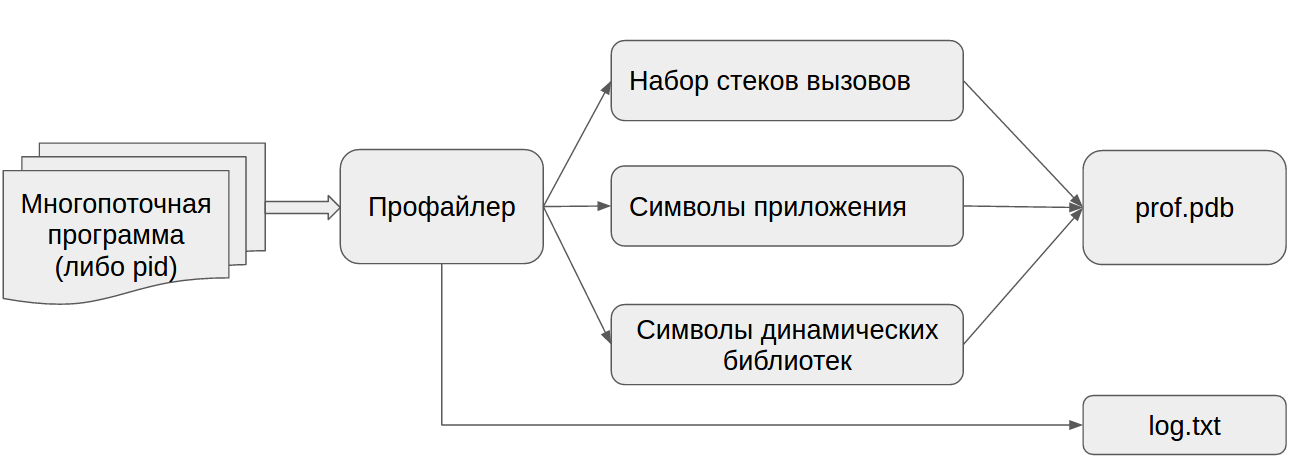
\includegraphics[width=\linewidth]{images/general_profiler}
    \end{figure}    
    
\section{Мониторинг запущенных потоков}
	Сбор стеков вызовов должен происходить для каждого потока отдельно, поэтому в этой секции будет рассказано про методы для мониторинга запущенных потоков. Если собирать всю информацию не выделяя каждый поток отдельно, получится перемешанная информация, которую сложно анализировать. Например, если пользователю интересны только некоторые из работающих потоков, ему будет удобнее посмотреть только на статистику внутри них, не показываю всю информацию о приложении. В языке C++ \cite{meyers} нет функции или простого способа для получения списка текущих потоков и мониторинга за ними. Далее будут показаны возможные решение их плюсы и недостатки.
    
    Для получения списка текущих потоков для приложения в Linux можно, например, перегрузив функцию \verb|pthread_create|. Так как она реализована в \verb|libpthread.so| можно подгрузить настоящую функцию при помощи \verb|dlopen| и заменить ее своей с добавлением \verb|tid| в специальный контейнер. С помощью этого можно мониторить создание потоков. Теперь только, чтобы подменить стандартную реализацию создания потоков на новую нужно скомпилировать ее как динамическую библиотеку. Пользователю для профилирования придется использовать подмену переменной окружения перед запуском \verb|LD_PRELOAD|, чтобы наша библиотека загрузилась раньше стандартной. Также данный подход не будет работать при статической сборке из-за этого он не подходит. Однако ровно так предлагают решить проблему с потоками в профайлере \verb|google-perftools|.
    
    Также можно воспользоваться утилитой \verb|ps| которая отображает текущие запущенные процессы и при помощи \verb|grep| найти нужные потоки. При использовании данного подхода было выявлено, что он очень медленно работает и сильно \enquote{тормозит} профайлер, так как список текущих потоков приходится брать каждый раз перед началом сбора стеков вызовов. 
    
    Третье решение наиболее удачно подошло для поставленной задачи. В Linux есть специальная файловая система \verb|procfs| которая представляет информацию о запущенных процессах. В разделе \verb|/proc/pid/task| можно найти информацию о всех потоках запущенных для данного pid. Сканируя данную директорию можно получить все необходимые идентификаторы потоков. Это приходится делать каждый раз перед сбором стеков вызовов, так как потоки могут завершаться и создаваться заново. По тестам проведенным в процессе написания профайлера было выявлено, что такой подход хорошо работает и почти не привносит дополнительных накладных расходов по сравнению с предыдущими.    
    
\section{Остановка потоков приложения}
	Чтобы развернуть стек вызовов для конкретного потока для начала нужно его остановить. Когда мы получили список идентификаторов всех потоков, нужно подключится к ним для возможности смотреть на их текущее состояние. Подключение к потокам осуществляется через системный вызов \verb|ptrace| при помощи \verb|PTRACE_ATTACH| иллюстрацию можно увидеть на рис. \ref{fig:ptrace_attach}. Подключившись к каждому потоку появляется возможность управлять его работой. Главный поток необходимо зарегистрировать на событие выхода при помощи \verb|PTRACE_SETOPTIONS|, чтобы профайлер узнал о том, что приложение собирается закрыться до того как оно очистило все свои ресурсы и выгрузило информацию о динамических библиотеках.
    
    \begin{figure}[H]
        \caption{Подключение к профилируемому приложению}
        \label{fig:ptrace_attach}
        \centering
        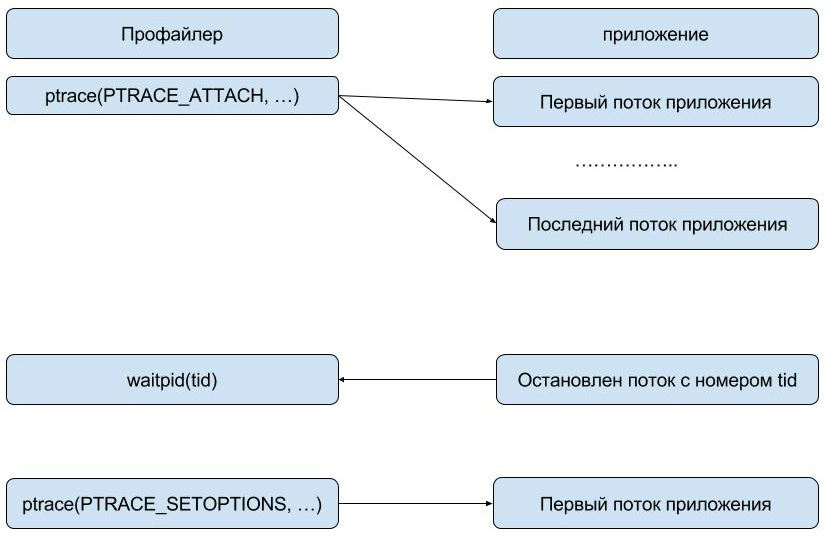
\includegraphics[width=\linewidth]{images/ptrace_attach}
    \end{figure}    
    
    Для остановки каждого потока используется отправка сигнала \verb|SIGSTOP| посредством системного вызова \verb|tkill|. Этот сигнал в системе Linux не может быть обработан или проигнорирован приложением. Он приостанавливает данный поток, после чего появляется возможность смотреть на его текущее состояние. Из-за того, что посылка сигнала происходит из другого приложения то он получается не мгновенно. Также поток может находится в очереди на исполнения, если их больше чем физических ядер. Поэтому сигнал может ему прийти не скоро и профайлер не должен останавливать свою работу из-за одного спящего потока. Для этого был реализован метод для асинхронной отправки сигнала и проверки, без ожидания, состояния всех потоков. В тот момент когда сигнал дойдет и поток действительно остановится можно начинать сбор информации о нем. После того как стек вызовов будет получен, этому потоку будет отправлен сигнал \verb|SIGCONT| для продолжения работы.
    
\section{Разворачивание стека вызовов}
	Получив доступ к стеку приложения и регистрам можно определить последовательность вызовов функций, которые привели в текущее состояние профилируемое приложение. В архитектуре \verb|x86_64| есть регистр RIP, который хранит адрес, указывающий на текущую выполняемую инструкцию. В бинарном файле приложения есть информация о том по каким адресам расположены функции программы и какой размер в байтах занимает их код. Благодаря этому можно понять текущую функцию исполнения и ассемблерную команду. Приложение при вызове функции кладет в стековый кадр адрес возврата и сохраняет в регистр EBP указатель на начало кадра, процедура показана на рисунке \ref{fig:call_stack}. Благодаря этому мы можем понять кто вызвал нашу функцию, посмотрев на адрес возврата и \enquote{прыгнув} по нему. После повторив данную процедуру мы получим стек вызовов приложения.
    
    \begin{figure}[H]
        \caption{Разворачивания стека потока приложения}
        \label{fig:call_stack}	
        \centering
        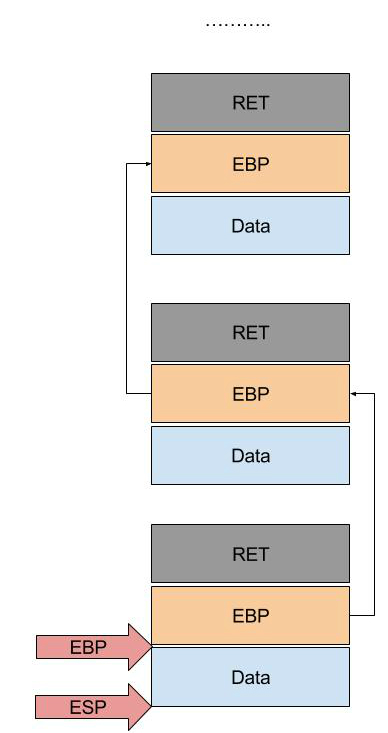
\includegraphics[scale=0.5]{images/call_stack}
    \end{figure}  
    
    Многие компиляторы при включении оптимизаций, например опцией \verb|-O2|, по умолчанию включает опцию \verb|-fomit-frame-pointer|, которая разрешает компилятору не сохранять в регистр EBP адрес на начало стекового кадра, для большей производительности. Из-за чего становится очень сложно получить стек вызовов. Поэтому большинство профайлеров требует от пользователей, чтобы они компилировали свои приложения, перед началом профилирования, с опцией \verb|-fno-omit-frame-pointer|, которая заставляет компилятор сохранять в регистр адрес на начало кадра.
    
    Сначала была написана своя функция по развертки стека вызовов, из-за простоты реализации и понимания происходящего. Но после было решено использовать библиотеку \verb|libunwind|. Она способна разматывать стек как с опцией сохранения EBP так и без него. Удается ей это сделать при помощи анализа отладочной информации хранящейся в бинарном файле. Однако по прежнему приложение желательно компилировать с опцией \verb|-fno-omit-frame-pointer| для более быстрого получения стека вызовов. Также наблюдались случаи, когда библиотека \verb|libunwind| неправильно разворачивала стек, если отсутствовала опция компилятора для сохранения информации о начале стекового кадра. В этой библиотеке присутствует возможность разворачивать стек удалено. Это можно делать только после того, как мы подключились к приложению и приостановили его работу.
        
\section{Сбор символов динамических библиотек}
	Динамическая библиотека сделана для загрузки в приложение во время запуска или во время исполнения, в отличии от статических которые нацелены, чтобы копироваться полностью в приложение, создавая монолитный исполняемый файл. Динамическая библиотека собирается с опцией компилятора \verb|-fPIC|, что создает независимый от размещения в памяти код. Все адреса функций в нем относительны, а не абсолютны, как это обычно бывает в бинарном файле. 
    
    \begin{figure}[H]
        \caption{Отображение динамических библиотек в приложении}
        \label{fig:dynamic_lib}
        \centering
        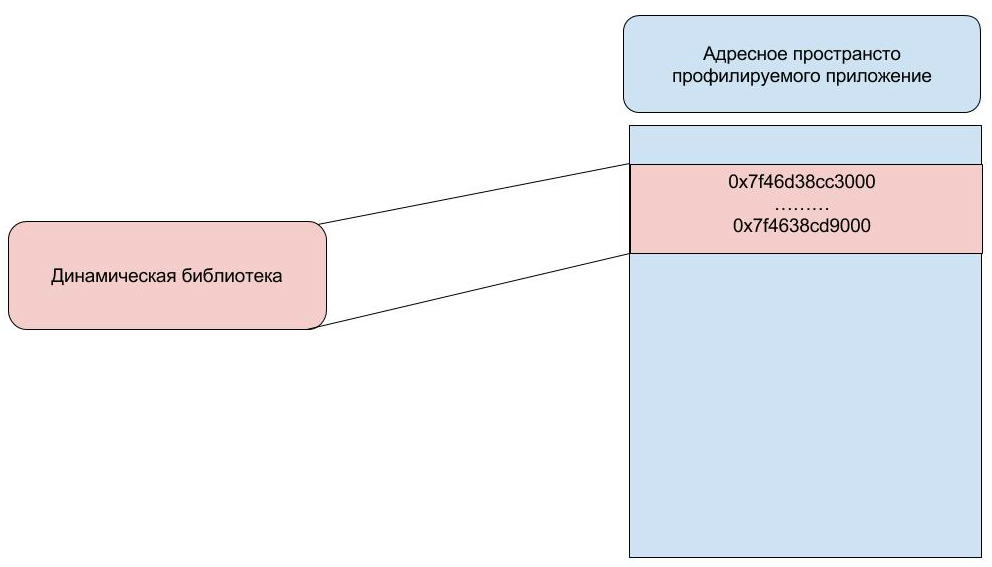
\includegraphics[width=\linewidth]{images/dynamic_lib}
    \end{figure} 
    
    Так как адреса функций в динамических библиотеках относительны, нужно узнать в каком диапазоне адресов была подгружена какая библиотека, пример на рисунке \ref{fig:dynamic_lib}. Эту информацию можно найти в файловой системе \verb|procfs|. В разделе \verb|/proc/pid/maps|. Пример строчки из этого файла:
\begin{lstlisting}
    7f46d38cc3000-7f4638cd9000  r-xp  ...  /lib/libc-2.23.so
\end{lstlisting}
    В ней можно увидеть в какой диапазон адресов загрузилась библиотека libc. Что она загрузилась на чтение и исполнение. После того как мы узнали по какому адресу находится библиотека, можно прочитав ее символы и относительные их адреса понять абсолютные адреса расположения объектов, которые будут подгружены в наше приложение.
    
    Для чтения символов исполняемого файла, использовалась утилита \verb|readelf|, которая может предоставить манглированные имена всех функций данного файла, адреса по которым они располагаются и размер в байтах который занимает функция. Изначально деманглирование символов происходило с помощью функции \verb|abi::__cxa_demangle(...)| предоставляемой библиотекой \verb|libstdc++|. Но в ходе работы было обнаружено, что деманглирование некоторых имен  с ее помощью работает неправильно. Так например если вызвать эту функции для вполне нормального имени функции \verb|g()|, то она его превратит в \verb|__float128()|. После этого было решено использовать утилиту \verb|c++filt| для деманглирования имен, которая не имеет такой проблемы. За время работы профайлера проблем с ней не возникло. Вся эта информация сохраняется в файл с собранными стеками вызовов перед завершением профилируемой программы, либо при получение сигнала \verb|SIGTERM|. 

    
\section{Скорость работы}
	Проводилось множество различных экспериментов и замеров накладных расходов профайлера на приложения. Одно из них представлено в листинге \ref{code:logger}. В программе работают два потока, один из них занимается тем, что берет данные из буфера и записывает их в файл, второй поток записывает данные в буфер и уведомляет второй, что появились новые данные. Эта программа интересна с точки зрения замеров профайлера в том плане, что в ней присутствует несколько потоков, а также большую часть времени она находится в блокировке под мьютексом. В ней производится множество запусков и считается среднее время. Измерения показали, что написанный профайлер замедляет данное приложение всего лишь на 3\%. Количество сэмплов было выставлено 100 в секунду, что вполне достаточно для показательного профиля в большинстве случаев. 
    
    Второе измерение производилось на программе представленной в \ref{code:writer}. На ней измерения показали ухудшений в производительности на 5\%. В сравнении с утилитой perf - она замедляла на 3\%.
    
    В процессе измерений было показано, что данный профайлер, хорошо справляется с поставленной задачей. Максимальное замедление, которое встречалось в процессе измерений было 10\%. 
        
\chapterconclusion
	В данной главе был описан алгоритм с помощью которого происходит сбор информации о профилируемом приложении. Были рассмотрены разные подходы и их проблемы к решению поставленной задачи. Были показаны замеры накладных расходов, накладываемых профайлером на приложение. В итоге был выбран наиболее подходящий алгоритм для сбора информации о запущенном приложении.
